%# -*- coding: utf-8-unix -*-
% !TEX program = xelatex
% !TEX root = ../thesis.tex
% !TEX encoding = UTF-8 Unicode
%%==================================================
%% chapter01.tex for SJTU Master Thesis
%%==================================================

%\bibliographystyle{sjtu2}%[此处用于每章都生产参考文献]
\chapter{肠道菌群纵向模式与早产儿坏死性小肠结肠炎研究}
\label{chap:nec}

\section{引言}
肠道菌群紊乱常常见于多种早产并发症,包括坏死性小肠结肠炎(Necrotizing Enterocolitis, NEC)和迟发性败血症(Late-Onset Sepsis)。前者是一种以小肠黏膜缺血性坏死为特征的疾病,与重度炎症、肠道产气菌侵袭、产气侵入肠道壁和门静脉系统相关\cite{neu2011necrotizing},在早产儿发病率为4~7\%\cite{rees2010national};起病快,进展凶险,严重者可致死。近年来有研究发现肠道菌群紊乱存在于NEC发病期间。后者是一种在出生后72小时后发生的败血症,其是早产儿和极低出生体重的死亡主要原因之一\cite{stoll2002late}。近期,有报道LOS患儿肠道内菌群多样性下降\cite{mai2013distortions},致病菌包括肠球菌(\textit{Enterococcus})丰度增加\cite{stewart2017longitudinal},提示肠道菌群紊乱与LOS发病相关。本研究拟自早产儿出生后纵向收集其粪便标本,标准化处理后进行二代测序,以探究肠道菌群定植模式发展对于NEC和LOS发病的贡献,为其预防治疗提供理论基础。

\section{材料与方法}
  \subsection{伦理}
  该研究经上海市儿童医学中心伦理联合委员会批准,上海交通大学医学院(SCMCIRB-K2013022)。 在从采集婴儿粪便样本之前,取得其监护人理解、同意并于知情同意书上签字。
  \subsection{研究对象}
  于2013年7月至2014年12月间,上海儿童医学中心新生儿重症监护病房(NICU)患儿,
    \subsubsection{入选及排除标准}
      \paragraph{入组标准}
      胎龄小于34周,出生体重不低于950g的住院患儿。
      \paragraph{排除标准}
      1)新生儿早发型败血症,2)肝脏疾病,3)肾功能损害(Cr>88μM),4)存在先天肠道发育异常,5)需要进行大型胸部或腹部手术(男性包皮环切术或PDA结扎除外),6)预计使用肠外营养(Parental Nutrition, PN)支持供应超过50%的每日卡路里摄入量,且时间超过4天,7)静脉注射抗生素(除头孢噻肟、哌拉西他唑和甲硝唑),8)有口服抗生素史,9)有血便史,10)日龄大于五天者。
  \subsection{诊断标准}
  关注每名患儿入院后的健康情况,评估并记录一般情况全身,腹部平片报告结果等,观察其是否发生NEC(II期和III期)或LOS。

  坏死性小肠结肠炎NEC诊断和分级根据“改良Bell分级标准(24)”:II期,伴有放射性肠扩张,肠梗阻,肠道积气和/或腹部压痛,和/或轻度代谢性酸中毒,肠鸣音减弱,血小板减少症。

  迟发型败血症LOS确诊标准:如果患儿在出生后72小时后,由至少两位新生儿科医生独立检查确认脓毒症体征/症状,血培养或其他体液培养阳性或可疑阳性,并接受过高级别抗生素治疗(例:美罗培南等),则诊断为LOS。

  无感染性并发症或败血症、NEC的患儿为对照组。

  \subsection{主要实验室试剂及仪器}
  \label{主要实验室试剂及仪器}
    \subsubsection{试剂与材料}
    \begin{enumerate}
      \item PowerSoil\textsuperscript{\textregistered} DNA Isolation Kit:美国MoBio公司
      \item AxyPrepDNA凝胶回收试剂盒: Axygen爱思进生物技术(杭州)公司
      \item TruSeq\textsuperscript{TM} DNA Sample Prep Kit:Illumina中国
      \item 纸质冻存管盒:江苏省中瑞实验器材经营部
      \item 冻存管(规格1.8ml):江苏省中瑞实验器材经营部
      \item 无菌塑料铲子:江苏省中瑞实验器材经营部
      \item 干冰:上海京日实业有限公司
    \end{enumerate}
    \subsubsection{仪器}
    \begin{enumerate}
      \item -80℃实验室冰箱(超低温冰箱):ThemoFisher赛默飞世尔科技(中国)有限公司
      \item 电子天平(型号XSE104):梅特勒-托利多国际贸易(上海)有限公司
      \item 恒温金属浴(型号TU-100C):上海一恒科学仪器有限公司
      \item 小珠研磨器MiniBeatbeater™(型号-16):美国BioSpec实验仪器设备公司。
      \item 台式高速冷冻离心机(型号5427R):Eppendorf艾本德(上海)国际贸易有限公司
      \item 移液器(型号:Eppendorf Reference® 2;规格:20 μl, 100 μl,200 μl L,1000 μl):Eppendorf艾本德(上海)国际贸易有限公司
      \item 移液器支架系统(The Eppendorf Pipette Holder System):Eppendorf艾本德(上海)国际贸易有限公司
      \item 自封式双层超滤芯吸头(型号Dualfilter T.I.P.S.® SealMax;规格:20 μl, 100 μl,200 μl,1000 μl):Eppendorf艾本德(上海)国际贸易有限公司
      \item 漩涡混合器(型号:VORTEX-5:江苏省海门市其林贝尔仪器制造有限公司
      \item 2-8℃医用冷藏箱(型号:HYC-940(F)):中国海尔集团
      \item 超微量紫外线分光光度计(型号NanoDrop 2000C):ThemoFisher赛默飞世尔科技(中国)有限公司
      \item PowerPac™ 通用电泳仪电源
      \item 水平小型电泳槽(型号:Sub-Cell® 96):BIO-RAD伯乐生命医学产品(上海)有限公司
      \item ABI GeneAmp® PCR仪(型号: 9700):ThemoFisher赛默飞世尔科技(中国)有限公司 美国应用生物系统中国公司
      \item Tanon 4100 全自动数码凝胶图像分析系统:上海天能科技有限公司
      \item QUANTIFLUOR™荧光计仪(型号QUANTIFLUOR™ST/P):Promega - 普洛麦格(北京)生物技术有限公司,上海盛兆生物科技有限公司。
      \item 16sRNA第二代高通量平台(Illumina Miseq):Illumina中国
    \end{enumerate}
  \subsection{粪便标本采集方法}
  \label{粪便标本采集方法}
    \begin{enumerate}
      \item 取得患儿监护人理解、同意并于知情同意书上签字。
      \item 准备无菌手套、干冰(置于密封盒中)、无菌塑料铲子、冻存管。
      \item 待患儿排便后,带手套,使用塑料铲子,于肛门周围皮肤或尿布附近刮取粪便样本,置于冻存管内,约 1g。
      \item 根据入组患儿编号和采集时间,对样本进行编号后立刻放入干冰盒中,30分钟内储存于-80℃冰箱中备用。
    \end{enumerate}

  \subsection{标本总DNA提取}
  \label{标本总DNA提取}
  本课题使用PowerSoil\textsuperscript{\textregistered} DNA Isolation Kit试剂盒(Catalog No. 12888-100)提取粪便标本总DNA;流程如下所述:
  操作全程都需带手套。
    \begin{enumerate}
      \item 向所提供的PowerBead管中加入不少于0.25克粪便标本(均质化和裂解程序,管内的缓冲剂将(a)帮助分散土壤颗粒,(b)开始溶解腐殖酸(c)保护核酸免于降解)
      \item 使用漩涡混合器,轻轻涡旋混合(开始将样品分散在PowerBead溶液中)。
      \item 检查溶液C1,如果观察到C1沉淀,将溶液置于恒温金属浴60°C直至沉淀物在使用前溶解。溶液C1可以在加热后直接使用。(溶液C1包含SDS和其他裂解细胞所需的阻断成分;SDS作为一种阴离子洗涤剂,也可帮助分解与细菌细胞膜相关的脂肪酸和脂质有关的脂肪酸。金属浴60°C将溶解SDS,但不会损害SDS或其他阻断成分。)
      \item 在PowerBead管中加入60μl溶液C1并手动翻转数次,或也可以短暂涡旋混合。
      \item 使用小珠研磨器MiniBeatbeater™垂直固定PowerBead管,以最大速度涡旋15分钟。(注意:1)标准时间为10分钟,但本课题使用24孔Beatbbeater™,故涡旋时间增加至15分钟;2)涡旋步骤对于完全均质化和细胞裂解是至关重要的。 通过来自步骤1-4的化学试剂和在该步骤引入的机械振荡的组合裂解细胞。 通过在破坏剂存在下随机摇动珠子,珠子与微生物细胞的机械震荡、碰撞将是的微生物细胞完全破裂。)
      \item 确保PowerBead管在离心机中无摩擦、可自由旋转。 在室温下以10,000xg离心1分钟。 (注意:1)转速不应超过10,000 x g,因为管子可能会破裂。2)标准流程离心时间为30秒,由于本课题所收取的样品量有时较多,经尝试,离心时间1分钟的离心效果较好。)
      \item 将第(6)步中收取的上清液转移至干净的2 ml收集管(试剂盒提供)中,该步骤上清液约500μl。
      \item 将250μl溶液C2加入步骤(7)中的收集管中,然后涡旋5秒;在4°C环境中孵育5分钟。(溶液C2为 Inhibitor Removal Technology®(IRT),含有一种沉淀非DNA有机和无机物质的试剂,包括腐殖质,细胞碎片和蛋白质,同时可去除可能降低DNA纯度并抑制下游DNA应用的污染性有机和无机物质。)
      \item 在室温下,离心步骤(8)中的收集管,转速10,000 x g,离心时间1分钟。
      \item 将步骤(9)中收取的上清液(体积不多于600μl的)转移至新的干净的2 ml收集管(试剂盒提供)中,注意吸头避免碰触沉淀。(此时的沉淀含有非DNA有机和无机物质,包括腐殖酸,细胞碎片和蛋白质。为了获得最佳的DNA产量和质量,请避免转移任何沉淀。)
      \item 将200μl溶液C3加入步骤(10)中的上清液中,并短暂涡旋。在4°C孵育5分钟。(溶液C3为 Inhibitor Removal Technology®,IRT),是另一种沉淀其他非DNA有机和无机物质的试剂,包括腐殖酸,细胞碎片和蛋白质,也可去除可能降低DNA纯度并抑制下游DNA应用的污染性有机和无机物质。
      \item 在室温下,离心步骤(11)中的收集管,转速10,000 x g,离心时间1分钟。
      \item 将步骤(12)中收取的上清液(体积不多于750μl的)转移至新的干净的2 ml收集管(试剂盒提供)中,注意吸头避免碰触沉淀。(此时的沉淀含有非DNA有机和无机物质,包括腐殖酸,细胞碎片和蛋白质。为了获得最佳的DNA产量和质量,请避免转移任何沉淀。)
      \item 使用溶液C4前,将其轻轻摇匀。将1.2ml溶液C4加入步骤(13)中的收集管中(此步骤小心缓慢,避免溶液溢出收集管边缘),然后涡旋5秒。(溶液C4是高浓度盐溶液。 由于DNA在高盐浓度下与二氧化硅紧密结合,因此C4可以调节DNA溶液盐浓度,以使DNA(但可能仍然有低水平的非DNA有机和无机物质)与离心过滤管Spin Filter的滤膜结合。)
      \item 转移675μl步骤(14)中获取的混合液,于离心过滤管Spin Filter中,然后于室温下离心Spin Filter,转速10,000 x g,离心时间1分钟,弃去下层离心液。重复上述步骤,直至步骤(14)中的混合液完全耗尽, 共3次。(此时,高浓度盐溶液中结合DNA,且被选择性结合至Spin Filter二氧化硅过滤膜上。)
      \item 将500μl溶液C5加入Spin Filter中,然后将其于室温下离心,转速10,000 x g,离心时间1分钟。(溶液C5是乙醇基的洗涤溶液,用于进一步清洁与Spin Filter的二氧化硅滤膜结合的DNA。 该洗涤溶液除去残留的盐,腐殖酸和其他污染物,同时使DNA保持与二氧化硅膜结合。)
      \item 弃去步骤(16)中的下层离心液(含有非DNA的无机和有机物质)。
      \item 于室温下,再次将Spin Filter离心,转速10,000 x g,离心时间1分钟。尽可能完全除去残留的溶液C5(乙醇基洗涤溶液),因为乙醇会干扰许多下游DNA步骤,如PCR,限制性消化和凝胶电泳。
      \item 小心将Spin Filter 置于新的干净的2ml收集管(试剂盒已提供)中,避免将任何溶液C5带入新收集管。
      \item 将100μl溶液C6小心加入Spin Filter的白色滤膜上,保证整个滤膜充分浸润超市,然后静置等待1~2分钟。(溶液C6可与滤膜中的高浓度盐溶液结合,促使DNA与盐溶液解离并洗脱。因此,本课题在此处选择将其滤膜于室温下静置等待1~2分钟,以确保DNA更大程度的解离,后续浓度更高而适合建库测序。)
      \item 在室温下,将步骤(20)中的Spin Filter和收集管离心,转速10,000 x g,离心时间1分钟。
      \item 弃去Spin Filter,得到粪便样本总DNA。
      \item DNA提取质控:利用超微量紫外线分光光度计(型号NanoDrop 2000C)检测DNA,目标浓度约50ng/ml。利用1\%琼脂糖凝胶电泳检测DNA提取质量。
      \item 将通过质控的DNA样本置于-80°C冰箱中上海美吉生物医药科技有限公司进行后续扩增。
    \end{enumerate}

  \subsection{总DNA 16s rDNA V3-V4可变区片段的扩增}
  \label{总DNA 16s rDNA V3-V4可变区片段的扩增}
  扩增区域为16 s rDNA V3-V4可变区,合成带有Illumina官方接头序列barcode的特异引物。扩增模版为上述提取的粪便样品总DNA。用338F (5’-ACTCCTACGGGAGGCAGCAG-3’)和806R (5’-GGACTACHVGGGTWTCTAAT-3’) 引物对V3-V4可变区进行PCR扩增,扩增程序为:95℃ 预变性3min,27个循环(95℃ 变性30s,55℃ 退火30s, 72℃ 延伸30s),最后72℃延伸 10min (PCR仪:ABI GeneAmp® 9700型)。扩增体系为20ul,4ul 5*FastPfu 缓冲液,2ul 2.5mM dNTPs, 0.8ul 引物(5uM), 0.4ulFastPfu 聚合酶;10ng DNA模板。PCR 采用TransGen AP221-02:TransStart Fastpfu DNA Polymerase;PCR仪为ABI GeneAmp® 9700型。
  扩增质控:为保证后续数据分析的准确性及可靠性,全部样品均按照正式实验条件进行,尽可能使用低循环数扩增,每例样本重复扩增3次,使用2\%琼脂糖凝胶回收PCR产物,利用AxyPrep DNA Gel Extraction Kit (Axygen Biosciences, Union City, CA, USA) 进行纯化,Tris-HCl洗脱,2\%琼脂糖电泳检测。为保证后续数据分析的准确性及可靠性,需满足两个条件,1) 尽可能使用低循环数扩增;2) 保证每个样本扩增的循环数一致。随机选取具有代表性的样本进行预实验,确保在最低循环数中使绝大多数样本能够扩增出浓度合适的产物。
  \subsection{荧光定量}
  \label{荧光定量}
  利用QuantiFluor™-ST (Promega, USA) 进行检测定量。然后根据每例DNA样本的目标测序量,进行相应比例的混合。
  \subsection{Illumina Miseq下一代高通量测序}
  \label{Illumina Miseq下一代高通量测序}
      \subsubsection{文库构建}
      根据Illumina MiSeq 平台 (Illumina, San Diego, USA)标准操作规程将纯化后的扩增片段构建PE 2*300的文库,构建步骤如下:
        \begin{enumerate}
          \item 连接“Y”字形接头;
          \item 使用磁珠筛选去除接头自连片段;
          \item 利用PCR扩增进行文库模板的富集;
          \item 氢氧化钠变性, 产生单链DNA片段,使用试剂TruSeqTM DNA Sample Prep Kit。
        \end{enumerate}
      \subsubsection{高通量测序}
      使用Illumina公司的Miseq PE300平台进行测序(上海美吉生物医药科技有限公司)
        \begin{enumerate}
          \item DNA片段的一端与引物碱基互补,固定在芯片上;
          \item 以DNA片段为模板,芯片上固定的碱基序列为引物进行PCR合成,在芯片上合成目标待测DNA片段;
          \item 变性、退火后,芯片上DNA片段的另一端随机与附近的另外一个引物互补,也被固定住,形成“桥(bridge)”;
          \item PCR扩增,产生DNA簇;
          \item DNA扩增子线性化成为单链。
          \item 加入改造过的DNA聚合酶和带有4种荧光标记的dNTP,每次循环只合成一个碱基;
          \item 用激光扫描反应板表面,读取每条模板序列第一轮反应所聚合上去的核苷酸种类;
          \item 将“荧光基团”和“终止基团”化学切割,恢复3'端粘性,继续聚合第二个核苷酸;
          \item 统计每轮收集到的荧光信号结果,获知模板DNA片段的序列。
        \end{enumerate}

  \subsection{原始数据处理}
  \label{原始数据处理}
  将测序所得的原始数据进行质控、过滤和优化后,进行OTU聚类和分类学水平注释。后续,本课题则基于OTU进行多种多样性指数分析,以及对测序深度的检测;基于分类学信息,在各个分类水平上,分析了样本所在的生物环境进行群落的组成、结构、相对丰度等特征。在上述分析的基础上,可以对多样本的群落组成和系统发育信息进行多元分析和差异显著性检验等一系列深入的统计学和可视化分析。
    \subsubsection{原始数据保存}
    为方便保存和共享各实验室产生的高通量测序数据,NCBI数据心建立了大容量的数据库SRA(Sequence Read Archive,http://www.ncbi.nlm.nih.gov/Traces/sra)来存放共享的原始测序数据。
    本实验的测序数据上传至NCBI数据库中(BioProject序列号:PRJNA470548)。
    \subsubsection{原始数据管理}
    根据序列索引中的barcode区分各个样本的数据,提取所需的数据后以fastq格式保存, PE数据每个样本有fq1和fq2两个文件,里面为测序两端的reads,且按顺序一一对应。

    Fastq(fq)是第二代测序技术中一种展示测序序列碱基质量的文件格式。每条序列read包含4行信息,其中:第一行为文件识别标志,第一行以“@”开头;第二行为具体的碱基序列;第三行为读段名(ID)(第三行中ID可以省略,但“+”不能省略),也可以含有文件识别标志;第四行是第二行中的序列内容每个碱基所对应的测序质量值,必须包含与序列中的字母相同数量的符号。

    如下所示:

    @HWI-ST531R:144:D11RDACXX:4:1101:1212:1946 1:N:0:ATTCCT

    (第一行)


    ATNATGACTCAAGCGCTTCCTCAGTTTAATGAAGCTAACTTCAATGCTGAGATCGTTGACGACATCGAATGGG

    (第二行)

    + HWI-ST531R:144:D11RDACXX:4:1101:1212:1946 1:N:0:ATTCCT

    (第三行)

    ?A\#AFFDFFHGFFHJJGIJJJIICHIIIIJJGGHIIJJIIJIIJIHGI@FEHIIJBFFHGJJIIHHHDFFFFDCCCCEDDCDDCDEACC

    (第四行)
    \subsubsection{接质控与优化数据}
    Illumina Miseq二代测序所得到原始数据PE reads序列为双端序列数据,根据序列件的重叠关系,将成对的reads拼接(merge)成一条序列,同时对reads的质量和merge的效果进行质控过滤,根据序列首尾两端的barcode和引物序列区分样品得到有效序列,并校正序列方向,即为优化数据。
    使用软件:Trimmomatic 软件质控,使用FLASH软件进行拼接。
    具体方法及相关参数:
      \begin{enumerate}
        \item 设置50bp的过滤窗口,如果窗口内的平均质量值低于20,从窗口前端位置截去该碱基后端所有序列,之后再去除质控后长度低于50bp的序列;
        \item  根据双段序列数据的正向和反向两条序列重叠关系(overlap)进行拼接(merge),拼接时overlap之间的最大错配率为0.2,长度需大于10bp。去除无法拼接的序列。
        \item 根据序列首尾两端的barcode和引物将序列拆分至每个样本,barcode需精确匹配,引物允许2个碱基的错配,去除存在模糊碱基的序列。
        \item 根据序列首尾两端的barcode和引物区分样品,并调整序列方向,barcode允许的错配数为0,最大引物错配数为2;
      \end{enumerate}
    \subsubsection{OTU聚类}
    在系统发生学或群体遗传学的研究中,为了便于进行分析,将某一个分类单元(例:品系,门,纲,目,属,种、分组等)人为地设置成同一标志,称为操作分类单元(Operational Unit Taxonomy,OTU)。当在科学研究中分析每个样本测序结果中的各水平分类单元的数目信息前,就需要对序列进行归类操作(cluster);通过这种归类操作,按照彼此的相似性将序列分归为许多小组,此时一个小组就是一个OTU。通常情况下,在97\%的相似水平下的OTU 进行生物信息统计分析。

    基于OTU可以进行多种多样性指数分析,基于OTU聚类分析结果,可以对样品生物群落进行多样性分析,并检测测序深度;基于分类学信息,则可以在各个分类水平上,对样本所在的生物环境进行群落的组成、结构、相对丰度等分析。在上述分析的基础上,可以对多样本的群落组成和系统发育信息进行多元分析和差异显著性检验等一系列深入的统计学和可视化分析。

    使用的UPARSE软件(version 7.1 http://drive5.com/uparse/) ,根据97\%的相似度对序列进行OTU聚类,并在聚类的过程中去除单序列和嵌合体。
    \subsubsection{分类学分析}
    为了得到每个OUT所对应的物种分类学信息,采用\href{RDP classifier}{http://rdp.cme.msu.edu/}贝叶斯算法对97\%相似水平的OUT代表序列进行分类学分析,并分别在各个分类学水平:

    domain(域),kingdom(界),phylum(门),class(纲),order(目),family(科),genus(属)比对\href{Silva数据库}{http://www.arb-silva.de},统计各样本的群落组成,默认置信度阈值为70\%。
    \subsubsection{多样性分析}
    多样性指数用来表述一个群落的多样性的统计量,在生物学中可以被用来描述某中环境下的生物多样性。多样性指数常备用来估算任何一个群落,每个成员都属于一个独特的群体或者物种。往往,多样指数的估计量存在一定的偏差,因此相似的值之间往往不能直接比较:本课题主要选择两个空间尺度来比较各分组间和样本间的微生物多样型——$\alpha$多样性和$\beta$多样性。

    $\alpha$多样性指数该指数主要关注局部均匀微生物群落的环境中的物种数目,在本课题中,该微生物群落基于特定分组或特定样本。它反映了群落内物种间通过竞争资源或者利用同一种群落环境而产生的共存结果,它可分为物种丰富度指数、物种均匀度指数和物种多样性指数。

    丰富度指数刻画了微生物群落中所含物种的多少,反映了一定空间范围内生物的丰富程度;其常常受制于群落总体包含的微生物数量,忽略了富集种和稀疏种对于群落多样性的贡献,因而常常将丰富度指数和均匀度指数结合使用。物种多样性指数则结合了物种多样性和多度性,本课题使用Shannon-Wienner指数(Shannon-wiener index)和Simpson多样性指数(Simpson’ diversity index)。其中,前者受物种丰富度和均匀度影响,该指数越大,则反映群落多样性越高,均匀度越低;后者反映了优势种在群落中的地位和作用,也成为生态优势度,与其他多样性指数呈负相关。多样性指数越高,生态优势度越小,均匀度指数越高:
      \begin{enumerate}
        \item Shannon-wiener index
          \begin{equation}
            \label{eq:shanon}
            H{'} = -\sum_{i=1}^{R}p_{i}\ln{p_{i}}\footnote{$p_i$属于第i种物种的个体数占群落中总个体数的比例。下同。}
          \end{equation}
        \item Simpson’ diversity index
          \begin{equation}
            \label{eq:simpson}
            D = \sum_{i=1}^{R}p_{i}^2
          \end{equation}
      \end{enumerate}

    $/beta$多样性指数该指数用来表示生物种类对于群落异质性的反映:不仅描述群落内不生物种类的数量,也考虑它们的相似性及其彼此之间的位置。通常$/beta$多样性表示为群落相似性指数或是同一分组内不同样本中生物物种的周转率。不同分组间生物种类的相似性越差,$/beta$生物多样性越高。

    本课题计算unweighed UniFrac distance, weighed UniFrac distance和Bray-Curtis dissimilarity来进行$/beta$多样性分析,其中weighed UniFrac distance将各物种丰度纳入考虑,而unweighed未对物种丰都进行加权处理。基于$/beta$多样性进行PCoA作图使用上述距离文件进行PCOA和PCA作图,每个代表一个样品菌群整体(即群落),而点与和之间的距离代表两个菌群整体(群落)间的序列相似度。

    PCA(Principal Components Analysis)即主成分分析,也称主分量分析或主成分回归分析法,首先利用线性变换,将数据变换到一个新的坐标系统中;然后再利用降维的思想,使任何数据投影的最大方差在第一个坐标(称为第一主成分)上,第二大方差在第二个坐标(第二主成分)上。这种降维的思想首先减少数据集的维数,同时还保持数据集的对方差贡献最大的特征,最终使数据直观呈现在二维坐标系。

    PCoA(Principal Co-ordinates Analysis)分析即主坐标分析,可呈现研究数据相似性或差异性的可视化坐标,是一种非约束性的数据降维分析方法,可用来研究样本群落组成的相似性或相异性。它与PCA类似,通过一系列的特征值和特征向量进行排序后,选择主要排在前几位的特征值,找到距离矩阵中最主要的坐标,产出结果是旋转后的数据矩阵,改变了坐标系统,并未改变样本点之间的相互位置关系。
    两者的区别为PCA是基于样本的相似系数矩阵来寻找主成分,而PCoA是基于距离矩阵(欧式距离以外的其他距离)来寻找主坐标。

  \subsection{统计学方法}
  \label{统计学方法}
    \begin{enumerate}
      \item 使用单因素方差分析和Kruskal-Wallis H test检验各水平物种在各组间的分布(相对丰度)是否存在显著性差异。
      \item 使用Student’s t检验评估两组间多样性指数的差异。若p < 0.05 则表示差异有统计学意义。过$\alpha$多样性分析可以得到群落(分组或者单个样本)中物种的丰度、覆盖度和多样性等信息。
      \item 利用Wilcoxon秩和检验,对每一组中的亚组进行两两检验,在具有显著差异物种类中的所有亚种比较是否都趋同于同一分类级别。
    \end{enumerate}

\section{结果}
  \subsection{患者基本情况}
  2013年7月至2014年12月,共有1148名早产儿入院,其中5名在此期间诊断为坏死性小肠结肠炎(NEC);发病率4.4%, 与总体发病率一致 [6] 。 在所有早产儿中,有130名符合我们的研究标准,并向其收集了1698份粪便标本。

  本研究最终选择24个充分采样的早产儿,包括4名坏死性小肠结肠炎(NEC)患儿(2个IIA期和2个IIB期),3个迟发型败血症LOS和17个匹配对照(表S1);共收集192个样本,其中NEC标本47个,LOS标本44个,对照组标本101个,并进行16s rRNA 基因测序。

  本研究中, 所有早产儿的平均胎龄为30.5周(28至33周),平均出生体重为1440克(945克至1950克)。 NEC组有3名女婴和1名男婴,LOS组有2名女婴和1名男婴,对照组有9名女婴和8名男婴。所有患儿均通过剖宫产分娩,并以早产儿配方奶喂养。 NEC的平均发病时间为出生后16天(范围:11至19天),确诊为LOS的平均生命日为12天。三组的人口统计学比较(表\ref{tab:necdemographic})显示,在胎龄,出生体重和性别百分比方面未见显著差异。

  \begin{table}[!hpb]
    \centering
    \bicaption[指向一个表格的表目录索引]
      {早产儿患者临床情况\footnotemark[1]}
      {Demographic characteristics of Preterm NEC, LOS and control groups.}
    \label{tab:necdemographic}
    \begin{tabular}{lp{1.8cm}p{1.8cm}p{1.8cm}p{2cm}c}
      \toprule
         & \textbf{NEC(n=3)} & \textbf{LOS(N=4)} & \textbf{Control(n-17)} & \textbf{Statistical Test} & \textit{p value} \\ \midrule
        \textbf{胎龄(周)} & 29(29-30) & 30(29-31) & 31(28-33) & Kruskal-Wallis test & 0.074 \\
        \textbf{出生体重(g)} & 1416.3 (773.4-2149.1) & 1141.7 (633.4-1649.9) & 1527.4 (1391.6-1663.1) & Kruskal-Wallis test & 0.111 \\
        \textbf{性别} &  &  &  & Fisher's test & 0.82 \\
        \multicolumn{1}{r}{女} & 3(75\%) & 2(\%67) & 9(\%53) &  & \\
        \multicolumn{1}{r}{男} & 1(25\%) & 1(\%33) & 8(\%47) &  & \\
        \textbf{诊断时年龄(天)} & 16(11-19) & 12(10-22) & — & Wilcoxon rank-sum test & 0.629 \\
        \textbf{住院时长(天)} & 54.3 (13.5-95.0) & 60.0 (24.8-95.2) & 32.9 (26.3-39.5) & Kruskal-Wallis test & 0.046 \\
        \textbf{标本总数} & 46 & 42 & 103 & — & — \\ \bottomrule
    \end{tabular}
  \end{table}
  \footnotetext[1]{NEC、LOS和对照组在入院时,胎龄、出生体重、年龄和性别无统计学差异。三组住院时常具有显著性差异(p = 0.046),这符合我们的预期,因为NEC和LOS患儿往往需要更长时间恢复,因此住院时间相对更长;比较NEC和LOS组住院时长未见明显统计学差异。胎龄=平均值(下限-下限),出生体重=平均值(95\%置信区间),诊断时年龄=平均值(下限-下限),性别=人数(占本组的百分比),住院时长=平均值(95\%置信区间)
  }

  一旦怀疑发生NEC,患儿会立即得到支持性护理和抗生素治疗——支持性护理包括停止肠内喂养、肠道休息,开始全肠外营养(TPN),补液,纠正代谢性酸中毒,肠道休息。在上海儿童医学中心新生儿重症监护病房,用于预防早产儿出生后败血症的抗生素组合为哌拉西林 - 他唑巴坦,头孢噻肟和甲硝唑。分别在治疗28天和15天后,两名NEC患儿情况好转并重新开始肠内喂养。一名婴儿在家人同意终止治疗并拒绝手术干预后死亡(表S1)。

  根据细菌血培养的阳性结果,来自LOS组的一名患儿被诊断出患有肺炎克雷伯菌菌血症,并且给予美罗培南21天;第二名患儿被诊断患有肺炎克雷伯氏菌和铜绿假单胞菌菌血症并给予美罗培南38天。第三名患儿被诊断为肺炎克雷伯菌菌血症、重症肺炎且对头孢噻肟耐药,因此给予美罗培南13天。

  住院前和住院期间所有患者均未接受接受益生菌处方。

  \subsection{样本及测序信息}
  入选NEC患儿4例,LOS患儿3例, 对照组患儿17例。采集其纵向粪便标本,共192个,其中NEC标本47个,LOS标本44个,对照组标本101个。其他临床资料见表表\ref{tab:necdemographic}。

  使用Illumina MiSeq高通量测序平台共测得 条16s rRNA基因序列,优化序列数目为7,472,400,优化碱基数目为3348,030,799,优化平均序列长度为448bp。

  \subsection{多样性分析}
    \subsubsection{$\alpha$多样性分析}
      \paragraph{NEC,LOS和对照组患儿件肠道菌群$\alpha$多样性分析}
      基于OTU进行计算,NEC,LOS和对照组Shannon-Wienner指数分别为:1.32,1.16和1.66;三组两两比较,可知LOS组和NEC组、NEC组和对照组shannon指数无统计学差异(分别p = 0.47,p = 0.06),LOS组和对照组之间存在统计学差异(p = 0.01)\ref{fig:2alphadiversity:shannon}。NEC,LOS和对照组Simpson指数分别为:1.32,1.16和1.66;三组两两比较,可知LOS组和NEC组Simpson指数无统计学差异(p = 0.77)、NEC组和对照组存在统计学差异(p = 0.03),LOS组和对照组之间存在统计学差异(p = 0.02)\ref{fig:2alphadiversity:simpson}。

      \begin{figure}[!htp]
        \centering
        \begin{minipage}[b]{0.6\textwidth} %标题宽度
          \centering
          \subcaptionbox{Shannon指数\label{fig:2alphadiversity:shannon}}
            {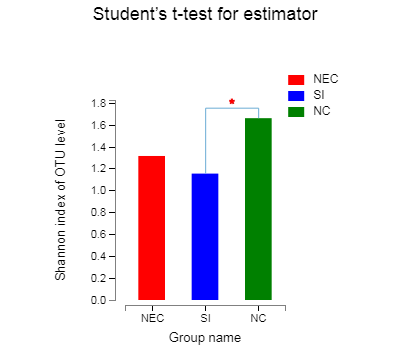
\includegraphics[height=5.5cm]{figure/2shannon.png}}
            \hspace{4em}
          \subcaptionbox{Simpson指数\label{fig:2alphadiversity:simpson}}
            {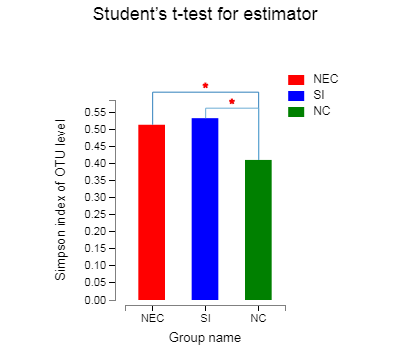
\includegraphics[height=5.5cm]{figure/2simpson.png}}
        \bicaption{通过计算Shannon指数(a)和Simpson(b)指数对NEC,LOS和对照组患儿件肠道菌群$\alpha$多样性分析}{Exploring $\alpha$ diversity by calculation Shannon diversity index(a) and Simpson diversity index(b) among preterm infants with NEC, LOS and Control groups.}
        \label{fig:2alphadiversity}
        \end{minipage}
      \end{figure}
      \subsection{$\beta$多样性分析}





\section{讨论}

\section{结论}
